
%-------------------------------------------------------------------------------------
% ESTA PLANTILLA REQUIERE UNA INSTALACION ACTUALIZADA DE TEXLIVE O MIKTEX (AL 2014)
%
% ACTUALICE TODA LA DISTRIBUCIÓN MIKTEX  O TEXLIVE ANTES DE USAR ESTA PLANTILLA
% O HAGA UNA REINSTALACIÓN DE LA DISTRIBUCIÓN
%
%  >>>>>  Esta plantilla requiere el paquete "psboxit" (está en esta carpeta: psboxit.sty) <<<<<<
%----------------------------------------------------------------------------------------


\documentclass[11pt,fleqn,x11names,table]{book}                                                  
% Dimensiones y márgenes.     
\usepackage[text={15cm,25cm},centering,headsep=20pt,top=0.8in,
bottom = 0.8in,letterpaper,showframe=false]{geometry} 

%----------------------------------------------------------------------
\input{Archivo_Diseno}% = Paquetes y código de diseño
%----------------------------------------------------------------------

\renewcommand{\tablename}{Tabla}
\definecolor{styrmitcrwcgray1}{rgb}{0.2,0.2,0.2}
\definecolor{wcgray}{rgb}{0,0.1333,0.3333}
\usetikzlibrary{arrows}

\usepackage{makeidx}
\makeindex
\usepackage{fourier} % Fuente global
% Insertar  páginas .pdf
\usepackage{pdfpages}


\begin{document}
% Insertar  Portada.pdf
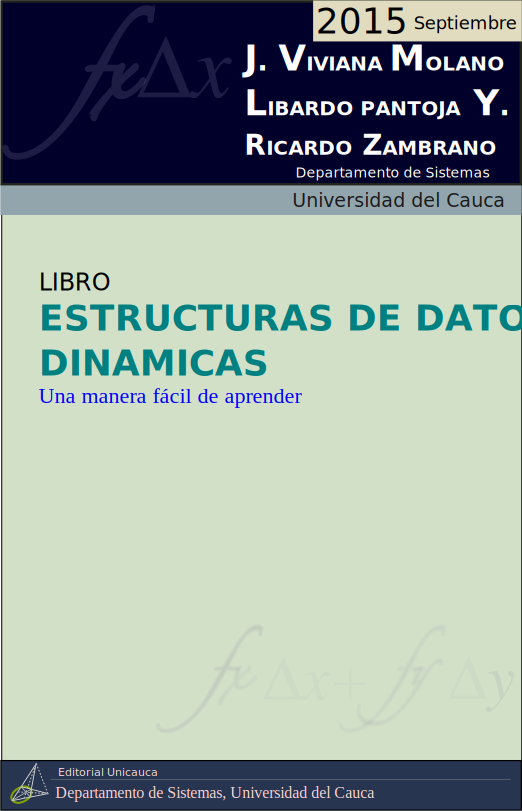
\includepdf[pages=-]{images/Portada}

\pagenumbering{roman} 
%\pagecolor{grisamarillo}
\parindent=0mm    % Sin sangría
\pagestyle{empty}
\titulo{% Autor (\fnte es un comando para un tipo de fuente especial)
       \huge\bfseries\color{wcolornotas} J. Viviana Mora., W Libardo Pantoja Y.}{%
        %pre-título
        \color{verdeF}Estructuras de Datos
        }{%
        %Título principal
         {\fontsize{80}{1} \selectfont Estructuras de Datos Dinámicas}
        }{%
        %Adicional
        Una forma fácil de aprender
        }

% %----------------------------------------------------------------------------------------
% % Página para "derechos reservados", ISBN, licencia creative commons, etc.
% %----------------------------------------------------------------------------------------
\clearpage
\begin{copyrightpage}{% 
   Universidad del Cauca (www.unicauca.edu.co). 
   Correo Electr\'onico: \url{editorial@unicauca.edu.co}
   Departamento de Sistemas
   Facultad de Ingeniería Electrónica y Telecomunicaciones
   Apdo. 159-7050, Popayán
   Teléfono (057)8209800
   Fax (058)8209900}%
Mora, Viviana.
\    Estructuras de Datos Dinámicas
\ W. Libardo Pantoja Yépez
\ -- Departamento de Sistemas, FIET, Universidad del Cauca.  2015.
\    xxx p.
\ ISBN 978-9977-66-227-5
\    1. Estructuras.  2. de Datos 3. Dinámicas.\\     
\end{copyrightpage}
~\vfill
%\thispagestyle{empty}

\noindent 
\parbox[s]{0.35\textwidth}{Licencia.}\parbox[c]{0.65\textwidth}{
 \color{gray}
 \fhv{9}{Revista digital}\\
 \fhvb{10}{Matemática, Educación e Internet.}\\
  \fntg[pag][9]{%
  \href{http://www.tec-digital.itcr.ac.cr/revistamatematica/}{http://www.tec-digital.itcr.ac.cr/revistamatematica/.}}
 }\\\\ % 

%\noindent {\color{colordominante} Photos by}: Viviana Loaiza. Parque Nacional Chirripó, Costa Rica.\\


\includegraphics[scale=0.7]{images/logocc}
\noindent  {{\fontsize{9}{1} \selectfont Este libro se distribuye bajo la licencia Creative Commons: Atribución-NoComercial-SinDerivadas CC BY-NC-ND (la "Licencia"). Usted puede utilizar este archivo de conformidad con la Licencia. Usted puede obtener una copia de la Licencia en 
\url{http://creativecommons.org/licenses/by-nc-nd/3.0/}.   En particular, esta licencia permite copiado y distribución gratuita, pero no permite venta ni modificaciones de este material.\\
  Límite de responsabilidad y exención de garantía: El autor o los autores han hecho su mejor esfuerzo en la preparación de este material.
  Esta edición se proporciona``tal cual''. Se distribuye gratuitamente con la esperanza de que sea útil, pero sin ninguna garantía expresa o implícita respecto a la exactitud o completitud del contenido.\\
  La Revista digital Matemáticas, Educación e Internet es una publicación electrónica. El material publicado en ella expresa la opinión de sus autores y no necesariamente la opinión de la revista ni la del Instituto Tecnológico de Costa Rica.}\\
  
  
%--------------------------------------------------------------------------------
%	Tabla de contenidos
%--------------------------------------------------------------------------------
\tableofcontents

%---------------------------------------------------------------------------------
% Prólogo
%---------------------------------------------------------------------------------

\begin{prologo}
\thispagestyle{empty}
Este texto  cubre aspectos básicos e intermedios sobre ipsúm dolor sit amet, consectetur adipiscing elit. Nam dignissim varius tempus. Cras eu malesuada ipsum. Pellentesque ut lorem velit. Mauris vehicula est orci, bibendum tincidunt enim mattis a. Interdum et malesuada fames ac ante ipsum primis in faucibus.. \\

 ...\\
 

    
\textit{Popayan, 2015.} \hfill{\sc V. Mora, W. Pantoja.}
\end{prologo}


\cleardoublepage
\pagestyle{fancy} % Habilitar encabezados
\pagenumbering{arabic}
\setcounter{page}{1}


%--------------------------------------------------------------------------------------
%	Capítulos
%---------------------------------------------------------------------------------------
%--------------------------------------------------------------------------------------
%	Capítulo 1
%---------------------------------------------------------------------------------------
\chapter{Capítulo 1: Contenido y Estilos en Latex}
Este capítulo sirve como modelo, es decir, para mostrar cómo utilizar latex. También muestra el posible contenido del libro. Un ejemplo de referencia bibliográfica es: \cite{kappel2006web}.


\begin{caja}[Advertencia.]
	Las siguientes plantillas usan la versión 2014 del paquete
	\verb+tcolorbox+ (entre otros paquetes recientes),  por lo tanto {\it debe actualizar los paquetes de sus distribución} \TeX{} o instalar manualmente este paquete (ver el capítulo 9 del libro, \url{http://www.tec-digital.itcr.ac.cr/revistamatematica/Libros/LATEX/LaTeX_2014.pdf}). El paquete "psboxit" viene incluido en la carpeta.
\end{caja}



%---------ESTRUCTURA GENERAL DEL LIBRO-------------_-
%------------------------------------------
\section{Estructura General del Libro}

\begin{enumerate}
	\item \textsc{Análisis de Algoritmos}
	\begin{enumerate}
		\item Los algoritmos
		\item El análisis de algoritmos
		\item Función de complejidad
		\item Cómo calcular la funcion de complejidad de un algoritmo
		\item Orden de Magnitud (Notación O Grande)
		\item Complejidad de un Algoritmo Recursivo
		\item Ejercicios Propuestos
	\end{enumerate}
	
	\item \textsc{Introduccion a las estructuras de datos}
	\begin{enumerate}
		\item Conceptos básicos sobre estructuras de datos.
		\item Clasificación.
		\begin{enumerate}
			\item Estructuras de Datos Estáticas.
			\item Estructuras de Datos Dinámicas.
		\end{enumerate}
	\end{enumerate}
	
	\item \textsc{Tipos abstractos de datos - TAD}
	\begin{enumerate}
		\item Tipos de datos
		\item Tipos abstractos de datos
		\item Métodos para la Especificación de un TAD
		\item Tipos de operaciones
		\item Ejemplos de TADs
		\item Ejercicios Propuestos
	\end{enumerate}
	
	\item \textsc{LISTAS DINÁMICAS}
	\begin{enumerate}
		\item Definición
		\item Usos de las listas
		\item El TAD Lista
		\item Implementación del TAD Lista orientado a objetos
		\item Implementación del TAD lista mediante arreglos
		\item Casos de estudio
		\item Ejercicios propuestos
	\end{enumerate}
	
	\item \textsc{PILAS}
	\begin{enumerate}
		\item Definición
		\item Usos de las pilas
		\item El TAD PIla
		\item Implementación del TAD pila orientado a objetos
		\item Implementación del TAD pila mediante arreglos
		\item Casos de estudio
		\begin{enumerate}
			\item Correspondencia de delimitadores
			\item Evaluación de expresiones aritméticas
			\item Convertir una expresión dada en notación infija a una notación postfija 
			\item Evaluación de la Expresión en notación postfija
		\end{enumerate}		
		\item Ejercicios propuestos
	\end{enumerate}
		
	\item \textsc{COLAS}
	\begin{enumerate}
		\item Definición
		\item Usos de las colas
		\item El TAD Cola
		\item Implementación del TAD cola orientado a objetos
		\item Implementación del TAD cola mediante arreglos
		\item Casos de estudio
		\begin{enumerate}
			\item Correspondencia de delimitadores
			\item Evaluación de expresiones aritméticas
			\item Convertir una expresión dada en notación infija a una notación postfija 
			\item Evaluación de la Expresión en notación postfija
		\end{enumerate}		
		\item Ejercicios propuestos
	\end{enumerate}		

	\item \textsc{Estructuras de Datos No Lineales. Arboles Binarios}
	\begin{enumerate}
		\item Introducción
		\item Definición de árbol
		\item Definición de árbol binario
		\item Árbol de expresiones
		\item Balance o equilibrio de un árbol binario
		\item Árbol binario completo
		\item TAD Árbol binario
		\item Implementación del TAD de un árbol binario
		\item Recorridos de un árbol
		\begin{enumerate}
			\item Recorrido inorden
			\item Recorrido en preorden
			\item Recorrido en postorden
			\item Recorrido en anchura
		\end{enumerate}		
		\item Árbol binario de búsqueda
		\begin{enumerate}
			\item Operación de inserción
			\item Operación de búsqueda
			\item Operación de eliminación
		\end{enumerate}	
		\item Árbol binario de búsqueda equilibrados AVL
		\begin{enumerate}
			\item Eficiencia en la búsqueda de un árbol equilibrado
			\item Inserción en árboles AVL
			\item Borrado de un nodo en un árbol AVL
		\end{enumerate}	
		\item Ejercicios propuestos
	\end{enumerate}	
			
	\item \textsc{Estructuras de Datos No Lineales. Arboles N-ARIOS}
	\begin{enumerate}
		\item Introducción
		\item Definiciones y conceptos básicos
		\item El TAD ArbolN
		\item Implementación del TAD ArbolN
		\item Ejercicios propuestos
	\end{enumerate}	
					
	\item \textsc{ARBOL1-2-3: UN ÁRBOL TRIARIO ORDENADO}
	\begin{enumerate}
		\item Introducción
		\item Definiciones
		\item El TAD ARBOL1-2-3
		\item Implementación del TAD ARBOL1-2-3
		\item Ejercicios propuestos
	\end{enumerate}			
	
	\item \textsc{ARBOL2-3: UN ÁRBOL TRIARIO ORDENADO}
	\begin{enumerate}
		\item Introducción
		\item Definiciones
		\item Un árbol B 
		\item El TAD ARBOL2-3
		\item Implementación del TAD ARBOL2-3
		\item Ejercicios propuestos
	\end{enumerate}
	
	\item \textsc{TRIE: CONJUNTO DE PALABRAS}
	\begin{enumerate}
		\item Introducción
		\item Definiciones
		\item El TAD TRIE
		\item Implementación del TAD TRIE
		\item Ejercicios propuestos
	\end{enumerate}	
	
	\item \textsc{CUADTREE: REPRESENTACIÓN DE IMÁGENES}
	\begin{enumerate}
		\item Introducción
		\item Definiciones
		\item El TAD CUADTREE
		\item Implementación del TAD CUADTREE
		\item Ejercicios propuestos
	\end{enumerate}	
	
	\item \textsc{Estructura dinámicas no lineales: Grafos}
	\begin{enumerate}
		\item Introducción
		\item Definiciones
		\item El TAD Grafo
		\item Representación de los Grafos
		\begin{enumerate}
			\item Matriz de adyacencia
			\item Implementación de la Matriz de Adyacencia
			\item Listas de adyacencia
			\item Implementación de la lista de Adyacencia
		\end{enumerate}	
		\item Recorridos de un Grafo
		\begin{enumerate}
			\item Recorrido en anchura
			\item Recorrido en profundidad
		\end{enumerate}			
		\item Conexiones en un grafo
		\begin{enumerate}
			\item Componentes conexas de un grafo
			\item Matriz de caminos, cierre transitivo
			\item Matriz de caminos y cierre transitivo
		\end{enumerate}	
		\item Matriz de caminos:Algoritmo de Warshall
		\item Algoritmo de costos mínimos:Dijkstra
		\item Algoritmo de Floyd
		\item Ejercicios propuestos
	\end{enumerate}							
								
\end{enumerate}		

\section{Prueba de entornos}

\begin{definicion}[(Igualdad)][cap1:Igualdad]
  $$a=b$$
\end{definicion}

\bigskip
Según la definición \ref{cap1:Igualdad}, la igualdad...\\

\bigskip
\begin{teorema}
 $$a=b$$
\end{teorema}

\bigskip
\begin{ejemplo}
 $$a=b$$
\end{ejemplo}

%------------------------------------------------------------------------------------------
\clearpage

\begin{lema}
  $$a=b$$
\end{lema}

\bigskip
\begin{corolario}
 $$a=b$$
\end{corolario}

\bigskip
\begin{caja}[Una caja de comentario]
 $$a=b$$
\end{caja}

\subsection{Tablas}
 % \usepackage{array,tabularx}
 % \usepackage[table, x11names]{xcolor}

\newcolumntype{Y}{>{\raggedleft\arraybackslash}X} % Ver tabularx
%
\tcbset{enhanced,fonttitle=\bfseries\large,fontupper=\normalsize\sffamily,
         colback=LightCyan1,colframe=DarkOrange4,colbacktitle=DarkOrange4,
         coltitle=black,center title
       }

%%-Tabla - Estilo beamer
\begin{tcolorbox}[tabularx={X||X||X},title= {\white Iteración}, beamer]
  & $x_i$           & $y_i=f(x_i)$ \\\hline\hline
A & $x_0=0$         & $0$           \\\hline
B & $x_1=0.75$      &  $-0.0409838$ \\\hline
C & $x_2=1.5$       &  $1.31799$  
\end{tcolorbox}


%EJEMPLO CODIGO FUENTE EN JAVA

\subsection{Ejemplo codigo fuente Java}

\begin{lstlisting}[language=Java]
package com.unicauca.ejemplo;
public class Hello {
//Comentario
/*Comentario*/
/**Comentario*/
public static void main(String[] args) {
System.out.println("Hola mundo");
}
}
\end{lstlisting}

%----------------------------------------------------------------------------------------
%	Capítulo 2
%----------------------------------------------------------------------------------------
\chapter{Capítulo 2. XXXXXXXX}

\section{Introduccion}

Lorem ipsúm dolor sit amet, consectetur adipiscing elit. Nam dignissim varius tempus. Cras eu malesuada ipsum. Pellentesque ut lorem velit. Mauris vehicula est orci, bibendum tincidunt enim mattis a. Interdum et malesuada fames ac ante ipsum primis in faucibus. Sed mi justo, facilisis eget eros at, tristique tempus metus. Suspendisse potenti. Vivamus sed tellus mollis, accumsan ipsum a, auctor ex. Duis ullamcorper quam ipsum. Donec ullamcorper porttitor pretium. Curabitur urna nunc, placerat sit amet et, fermentum vehicula purus. Pellentesque eget mi ex \cite{Chevalereau2}.

\subsection{Ejemplo codigo fuente Java}

\begin{lstlisting}[language=Java]
package com.unicauca.ejemplo;
public class Hello {
   //Comentario
   /*Comentario*/
   /**Comentario*/
   public static void main(String[] args) {
      System.out.println("Hola mundo");
  }
}
\end{lstlisting}



\noindent
Ahora compila usando \texttt{javac}:



\begin{lstlisting}[numbers=none]
$ javac HolaMundo.java
\end{lstlisting}
\include{Capitulos/Capitulo3}
\chapter{Pilas}

\section{Definición de Pila}
Una pila (stack en inglés) es una lista ordinal o estructura de datos en la que el modo de acceso a sus elementos es de tipo LIFO (del inglés Last In First Out, último en entrar, primero en salir) que permite almacenar y recuperar datos. Se aplica en multitud de ocasiones en informática debido a su simplicidad y ordenación implícita en la propia estructura. 

La Figura  \ref{fig:pila-diagrama-clases} muestra la representación gráfica de una pila con sus operaciones fundamentales de apilar (push en inglés) y desapilar o retirar (pos en inglés.).

La pila es muy útil en situaciones cuando los datos deben almacenarse y luego recuperarse en orden inverso.

\begin{figure}
	\centering
		\includegraphics{images/RepresentacionPila}
	\caption{Representación de una Pila}	
	\label{fig:pila-representacion}
\end{figure}

\begin{definicion}[Pila][capPilas:pila]
Una pila (stack en inglés) es una lista ordinal o estructura de datos en la que el modo de acceso a sus elementos es de tipo LIFO (del inglés Last In First Out, último en entrar, primero en salir) que permite almacenar y recuperar datos. FALTA REFERENCIA
\end{definicion}

\section{El TAD Pila}
A continuación se especifica el TAD de la Pila con sus operaciones fundamentales. Las operaciones apilar y desapilar son las más importantes. En seguida la especificación de cada operación del TAD al estilo C.

\begin{lstlisting}[numbers=none, language=C]
TAD Pila [ T ]
{ invariante: TRUE }
Constructoras:
   crearPila: 
Modificadoras:
	apilar: Pila T 
	desapilar: Pila
Analizadoras:
	cima: Pila 
	esVacia: Pila
Destructora:
	destruirPila: Pila

Pila crearPila( void )
/* Crea una pila vacia */
{ post: crearPila =  }

void apilar(Pila pil, T elem)
/* Coloca sobre el tope de la pila el elemento elem */\
{ post: pil = e1, e2, .. elem}

void desapilar(Pila pil)\\
/* Elimina el elemento que se encuentra en el tope de la pila */\\
{ pre: pil =e1, e2, ..en, n > 0 }
{ post: pil =e1, e2, .., en-1 }

T cima(Pila pil )
/* Retorna el elemento que se encuentra en el tope de la pila */
{ pre: n > 0 }
{ post: cima = en }

int esVacia( Pila pil )
/* Informa si la pila esta vacia */
{ post: esVacia = ( pil = ) }

void destruirPila( Pila pil )
/* Destruye la pila retornando toda la memoria ocupada */
{post: pil ha sido destruida }
\end{lstlisting}

\section{Implementación del TAD en Java}
A continuación se muestra una implementación en Java del TAD Pila. Debido a que es una Pila dinámica se utilizan nodos enlazados.  La Figura \ref{fig:pila-digrama-clases} muestra el diagrama de clases.


\begin{figure}
	\centering
		\includegraphics{images/DiagramaClases-Pila}
	\caption{Diagrama de clase de la implementación del TAD Pila}	
	\label{fig:pila-diagrama-clases}
\end{figure}

La implementación involucra básicamente dos clases: Nodo y Pila. 

\begin{lstlisting}[language=Java]
package co.unicauca.pilas;
public class Nodo<T> {
	//Atributo valor de tipo T. Almacena la referencia al objeto que se guarda en el nodo
 	private T valor;
 	//Referencia al siguiente nodo enlazado
 	Nodo<T> siguiente;
	//Constructor por defecto
 	public Nodo() {
 		valor = null;
 		siguiente = null;
 	}
	//Devuelve el valor 
 	public T getValor() {
 		return valor;
 	}
	//Modifica el valor
 	public void setValor(T valor) {
 		this.valor = valor;
 	}
	//Devuelve el atributo siguiente
 	public Nodo<T> getSiguiente() {
 		return siguiente;
 	}
	 //Modifica el atributo siguiente
 	public void setSiguiente(Nodo<T> siguiente) {
 		this.siguiente = siguiente;
 	}
 }
\end{lstlisting}
La clase Nodo representa cada uno de los nodos enlazados que almacenan los objetos que se apilan. Tiene dos atributos, el \textsl{valor} representa el valor que guarda el nodo (línea 4), en este caso es una referencia a un objetivo de tipo T (siendo T un tipo genérico). El atributo \textsl{siguiente} (línea 6), representa la referencia al siguiente nodo. Los demás son únicamente, constructor y getters y setters de cada atributo.

\begin{lstlisting}[language=Java]
package co.unicauca.pilas;
public class Pila<T> {
    //Atributo cabeza, que apunta al tope la pila
 	private Nodo<T> cabeza;
 	//Almacena el total de elemento de la pila
 	private int tamanio;
    //Constructor por defecto
 	public Pila() {
 		cabeza = null;
 		tamanio = 0;
 	}
	//Devuelve el total de elementos de la pila
 	public int getTamanio() {
 		return tamanio;
 	}
	//Verifica si la pila esta vacia
 	public boolean esVacia() {
 		return (cabeza == null)
 	}
	//Apila un elemento nuevo
 	public void apilar(T valor) {
	 	//Crear un nuevo Nodo
 		Nodo<T> nuevo = new Nodo<T>();
	 	//Fijaer el valor dentro del nodo
 		nuevo.setValor(valor);
 		if (esVacia()) {
	 		//Cabeza apunta al nodo nuevo
 			cabeza = nuevo;
 		} else {
	 		//Se enlaza el campo siguiente de nuevo con la cabeza
 			nuevo.setSiguiente(cabeza);
 			//La nueva cabeza de la pila pasa a ser nuevo
 			cabeza = nuevo;
 		}
 		//Incrementa el tamanio porque hay un nuevo elemento en la pila
 		tamanio++;
 	}
	//Elimina un elemento de la pila
 	public void retirar() {
 		if (!esVacia()) {
 			cabeza = cabeza.getSiguiente();
 			tamanio--;
. 		}
 	}
	//Devuelve el elemento almacenado en el tope de la pila
 	public T cima() {
 		if (!esVacia())
 			return cabeza.getValor();
 		else
 			return null;
 	}
 }
\end{lstlisting}

La clase Pila representa la pila como tal con sus operaciones principales de \textsl{apilar} y \textsl{retirar}. 

A continución el código de un Cliente que instancia la Pila que hemos creado. En este caso se almacenan objetos de tipo entero, se apilan algunos números, se imprimen los valores del tope de pila y se desapilan elementos.

\begin{lstlisting}[language=Java]
package co.unicauca.pilas;
public class ClienteMain {
	public static void main(String[] args) {
		//Crear una nueva pila de enteros
		Pila<Integer> pila2 = new Pila<Integer>();
		//Se apilan algunos datos enteros
		pila2.apilar(2);
		pila2.apilar(5);
		pila2.apilar(7);
		System.out.println("El tope de la pila es: " + pila2.cima());
		//Se desapila
		pila2.retirar();
		System.out.println("El tope de la pila es: " + pila2.cima());
		//Se desapila
		pila2.retirar();
		System.out.println("El tope de la pila es: " + pila2.cima());
		//Se desapila, como la pila esta vacia devuelve null
		pila2.retirar();
		System.out.println("El tope de la pila es: " + pila2.cima());
 		//Probar con otra pila, donde se almacenen objetos
 	}
}
\end{lstlisting}

La salida de este programa sería la siguiente.

\begin{lstlisting}[numbers=none]
El tope de la pila es: 7
El tope de la pila es: 5
El tope de la pila es: 2
El tope de la pila es: null
\end{lstlisting}


\chapter{Arboles Binarios}

\section{Conceptos generales}
Un arbol es una estructura daksfjaksdjf kajf kdafasd
f dajf sdaf as
f asdf dsafk asdkf sdaf adf dasf  ak sdfasdf asdfas f
asd fadf 
df.


\section{Tipos de arboles}

\subsection{Arboles binarios}

\subsection{Arboles AVL}

\begin{lstlisting}[language=Java]
package com.unicauca.ejemplo;
public class ArbolBianrio {
   //Comentario
   /*Comentario*/
   /**Comentario*/
   public static void main(String[] args) {
      System.out.println("Hola mundo");
  }
}
\end{lstlisting}

%----------------------------------------------------------------------------------------
%	Bibliografía
%----------------------------------------------------------------------------------------
\renewcommand\refname{\Large {Bibliograf\'ia}\vspace{1cm}} 
\addcontentsline{toc}{section}{\numberline{}Bibliograf\'{\i}a}
\bibliographystyle{IEEEtran}
\bibliography{IEEEabrv,../../biblio/BibPhD}{}

%----------------------------------------------------------------------------------------
%	Apéndices
%----------------------------------------------------------------------------------------

%\input{apendiceAgregarPaquetesNuevos.tex}
%\input{Habilitarshellescape.tex}
% \input{ApendiceA.tex}%insalar una distribución y un editor
% \input{softwareadicional}
% \input{massoftwareadicional}
% \input{ApendiceB.tex}
% \input{IndiceComun.tex}
% 
% %%%%%%%%%%% ImprimirIndice
%\printindex

\end{document}
